\section{VCO: Voltage Controlled Oscillator}
Esta secci\'on se propone el dise\~no de un oscilador de se\~nales senoidales cuya frecuencia pueda ser controlada por una tensi\'on de entrada,
de forma tal que para un dado rango de tensiones, se pueda producir la se\~nal deseada que var\'ie en un rango esperado de frecuencias.
En la Fig. \ref{fig:esquema_general_ejercicio_3} se ilustra un esquema general del sistema deseado.

\begin{figure}[H]
    \centering
    \includegraphics[scale=0.6]{../EJ3/Recursos/system_scheme.png}
    \caption{Esquema general del sistema propuesto}
    \label{fig:esquema_general_ejercicio_3}
\end{figure}


\subsection{Introducci\'on te\'orica}
El objetivo de esta introducci\'on es establecer las bases te\'oricas sobre las cuales se construye
el an\'alisis desarrollado para el dise\~no del sistema propuesto. No obstante, se asume que el lector posee
una base te\'orica sobre algunos conceptos, lo cual se ir\'a indicando a lo largo de tal an\'alisis.

\subsubsection{Distorsi\'on Arm\'onica}
La teor\'ia de series generalizadas de Fourier establece que cualquier se\~nal peri\'odica, es decir una funci\'on dada tal que
$f: I\!R -> I\!R$ que cumple tener un per\'iodo fundamental dado $f(t + T) = f(t)$, con T perteneciente a los reales positivos, puede
ser proyectada sobre un espacio vectorial descripto por su base ortonormal.
En otras palabras, la serie trigonométrica de Fourier como caso particular permite describir un se\~nal peri\'odica como combinaci\'on 
lineal de funciones seno y coseno. Se suele denominar a cada una de estas componentes como arm\'onicos cuyas frecuencias son m\'ultiplos de la 
frecuencia fundamental, y desde un punto de vista espectral es sencillo observar la distribuci\'on de potencia de la se\~nal para cada frecuencia
arm\'onica.

\begin{figure}[H]
    \centering
    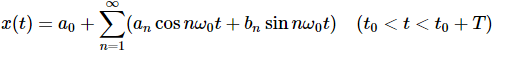
\includegraphics[scale=0.6]{../EJ3/Recursos/fourier_series.PNG}
    \caption{Series de Fourier}
\end{figure}


\begin{figure}[H]
    \centering
    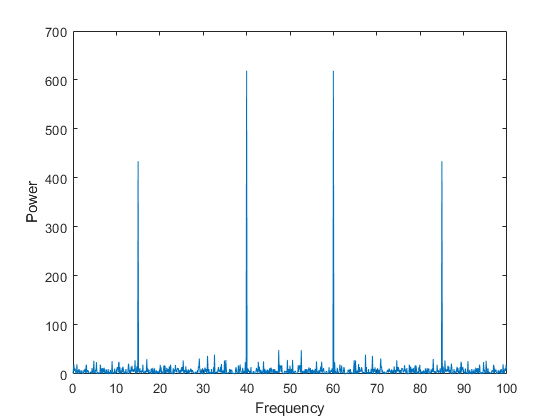
\includegraphics[scale=0.45]{../EJ3/Recursos/BasicSpectralAnalysisExample_01.png} 
    \caption{Espectro en frecuencia}
\end{figure}

La distorsi\'on arm\'onica puede ser entendida como la presencia de arm\'onicos no deseados que en el dominio temporal alteran o distorsionan la forma
de onda esperada, esto puede pasar como consecuencia del uso de sistemas no lineales o por el l\'imite f\'isico de ancho de banda que suelen tener
los circuitos, aunque no siempre se vuelve apreciable su efecto sobre la eliminaci\'on de los arm\'onicos deseados.
As\'i, una se\~nal senoidal pura \'unicamente contiene su arm\'onico fundamental, y en t\'erminos del espectro en frecuencia s\'olo una componente. Esto permite
estudiar la distorsi\'on de tales se\~nales analizando aquellos componentes arm\'onicos no deseados que pueden aparecen, y se utiliza la expresi\'on de la Ec. \ref{eq:distorsion_de_armonico}
para cuantificarla. La distorsi\'on total se define como se observa en la Ec. \ref{eq:total_distorsion}.

\begin{equation}
    HD_n = \frac{armonico_n}{armonico_{fundamental}}
    \label{eq:distorsion_de_armonico}
\end{equation}

\begin{equation}
    THD = \sqrt{\sum_{n} (HD_n)^{2}}
    \label{eq:total_distorsion}
\end{equation}

\subsubsection{Distorsi\'on de jitter}

\subsubsection{Explicaci\'on conceptual de un VCO}

\subsubsection{Explicaci\'on conceptual del conversor}

\subsection{An\'alisis de circuitos}

\subsubsection{Acondicionamiento lineal de se\~nal}
% Deducción y explicación del circuito para hacer el acondicionamiento
% lineal deseado

\subsubsection{Comparador Schmitt Trigger inversor}
% Explicar el Schmitt Trigger y sus cuentas

\subsubsection{Voltage Controlled Oscillator}
% Explicar el VCO y sus cuentas

\subsubsection{Conversor triangular a senoidal}
% Explicación del circuito!!

\subsection{Dise\~no de VCO}

\subsubsection{Especificaciones y etapas}

\subsubsection{C\'alculo de componentes}

\subsubsection{Simulaci\'on y verificaci\'on}

\subsection{Resultados}

\subsubsection{Mediciones}

\subsubsection{An\'alisis de resultados}

\subsection{Conclusiones}